%
% codebsp.tex -- Codierung eines Beispiels
%
% (c) 2021 Michael Steiner, Hochschule Rapperswil
%
\section{Codierung eines Beispiels
\label{reedsolomon:section:codebsp}}

Um die Funktionsweise eines Reed-Solomon-Codes besser zu verstehen, werden wir die einzelnen Probleme und ihre Lösungen anhand eines Beispiels betrachten.
Da wir in endlichen Körpern rechnen, werden wir zuerst solch einen Körper festlegen. Dabei müssen wir die Definition \ref{buch:endlichekoerper:def:galois-koerper} berücksichtigen, die besagt, dass nur Primzahlen für endliche Körper in Frage kommen.
Wir legen für unser Beispiel den endlichen Körper $\mathbb{F}_{q}$ mit $q = 11$ fest.
Zur Hilfestellung beim Rechnen in $\mathbb{F}_{11}$ können die beiden Tabellen \ref{reedsolomon:subsection:adtab} und \ref{reedsolomon:subsection:mptab} hinzugezogen werden. Diese Tabellen enthalten die Resultate der arithmetischen Operationen im Körper $\mathbb{F}_{11}$, die durchgeführt werden können.
Aus der Definition der endlichen Körper (ersichtlich auch in den Tabellen) folgt, dass uns nur die Zahlen \[\mathbb{F}_{11} = \{0,1,2,3,4,5,6,7,8,9,10\}\] zur Verfügung stehen und somit $11 = 0$ gelten muss.

\rhead{Codierung eines Beispiels}
% OLD TEXT
%Alle folgenden Berechnungen wurden mit den beiden Restetabellen \ref{reedsolomon:subsection:adtab} und \ref{reedsolomon:subsection:mptab} durchgeführt.
%Aus den Tabellen folgt auch, dass uns nur die Zahlen \[\mathbb{F}_{11} = \{0,1,2,3,4,5,6,7,8,9,10\}\] zur Verfügung stehen.

% die beiden Restetabellen von F_11
%%
% restetabelle1.tex -- Restetabelle von F_11: Addition
%
% (c) 2021 Michael Steiner, Hochschule Rapperswil
%

% alternatives design
%\begin{figure}
%\begin{center}
%\begin{tabular}{|>{$}c<{$}|>{$}c<{$}>{$}c<{$}>{$}c<{$}>{$}c<{$}>{$}c<{$}>{$}c<{$}>{$}c<{$}>{$}c<{$}>{$}c<{$}>{$}c<{$}>{$}c<{$}|}
%\hline
%+&0&1&2&3&4&5&6&7&8&9&10\\
%\hline
%0&0&1&2&3&4&5&6&7&8&9&10\\
%1&1&2&3&4&5&6&7&8&9&10&0\\
%2&2&3&4&5&6&7&8&9&10&0&1\\
%3&3&4&5&6&7&8&9&10&0&1&2\\
%4&4&5&6&7&8&9&10&0&1&2&3\\
%5&5&6&7&8&9&10&0&1&2&3&4\\
%6&6&7&8&9&10&0&1&2&3&4&5\\
%7&7&8&9&10&0&1&2&3&4&5&6\\
%8&8&9&10&0&1&2&3&4&5&6&7\\
%9&9&10&0&1&2&3&4&5&6&7&8\\
%10&10&0&1&2&3&4&5&6&7&8&9\\
%\hline
%\end{tabular}
%\end{center}
%\end{figure}

\begin{center}

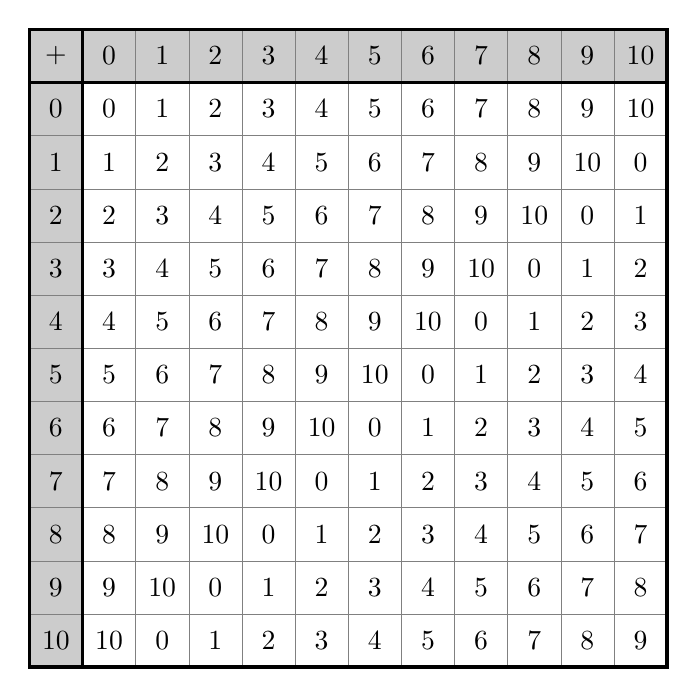
\begin{tikzpicture}[>=latex,thick,scale=0.45]
\fill[color=gray!40] (0,0) rectangle (18,-1.5);
\fill[color=gray!40] (0,0) rectangle (1.5,-18);	
\draw[step = 1.5, gray,very thin] (0,0) grid (18,-18);
\draw[very thick] (0,0) rectangle (18,-18);
\draw[very thick] (0,-1.5) -- (18,-1.5);
\draw[very thick] (1.5,0) -- (1.5,-18);
\node at (0.75,-0.75) {$+$};
\foreach \x in {0,...,10}
	\node at (2.25+\x*1.5,-0.75) {$\x$};
\foreach \y in {0,...,10}
	\node at (0.75,-2.25+\y*-1.5) {$\y$};
% Row 0
\node at ( 2.25,-2.25) {$0$};
\node at ( 3.75,-2.25) {$1$};
\node at ( 5.25,-2.25) {$2$};
\node at ( 6.75,-2.25) {$3$};
\node at ( 8.25,-2.25) {$4$};
\node at ( 9.75,-2.25) {$5$};
\node at (11.25,-2.25) {$6$};
\node at (12.75,-2.25) {$7$};
\node at (14.25,-2.25) {$8$};
\node at (15.75,-2.25) {$9$};
\node at (17.25,-2.25) {$10$};
% Row 1
\node at ( 2.25,-3.75) {$1$};
\node at ( 3.75,-3.75) {$2$};
\node at ( 5.25,-3.75) {$3$};
\node at ( 6.75,-3.75) {$4$};
\node at ( 8.25,-3.75) {$5$};
\node at ( 9.75,-3.75) {$6$};
\node at (11.25,-3.75) {$7$};
\node at (12.75,-3.75) {$8$};
\node at (14.25,-3.75) {$9$};
\node at (15.75,-3.75) {$10$};
\node at (17.25,-3.75) {$0$};
% Row 2
\node at ( 2.25,-5.25) {$2$};
\node at ( 3.75,-5.25) {$3$};
\node at ( 5.25,-5.25) {$4$};
\node at ( 6.75,-5.25) {$5$};
\node at ( 8.25,-5.25) {$6$};
\node at ( 9.75,-5.25) {$7$};
\node at (11.25,-5.25) {$8$};
\node at (12.75,-5.25) {$9$};
\node at (14.25,-5.25) {$10$};
\node at (15.75,-5.25) {$0$};
\node at (17.25,-5.25) {$1$};
% Row 3
\node at ( 2.25,-6.75) {$3$};
\node at ( 3.75,-6.75) {$4$};
\node at ( 5.25,-6.75) {$5$};
\node at ( 6.75,-6.75) {$6$};
\node at ( 8.25,-6.75) {$7$};
\node at ( 9.75,-6.75) {$8$};
\node at (11.25,-6.75) {$9$};
\node at (12.75,-6.75) {$10$};
\node at (14.25,-6.75) {$0$};
\node at (15.75,-6.75) {$1$};
\node at (17.25,-6.75) {$2$};
% Row 4
\node at ( 2.25,-8.25) {$4$};
\node at ( 3.75,-8.25) {$5$};
\node at ( 5.25,-8.25) {$6$};
\node at ( 6.75,-8.25) {$7$};
\node at ( 8.25,-8.25) {$8$};
\node at ( 9.75,-8.25) {$9$};
\node at (11.25,-8.25) {$10$};
\node at (12.75,-8.25) {$0$};
\node at (14.25,-8.25) {$1$};
\node at (15.75,-8.25) {$2$};
\node at (17.25,-8.25) {$3$};
% Row 5
\node at ( 2.25,-9.75) {$5$};
\node at ( 3.75,-9.75) {$6$};
\node at ( 5.25,-9.75) {$7$};
\node at ( 6.75,-9.75) {$8$};
\node at ( 8.25,-9.75) {$9$};
\node at ( 9.75,-9.75) {$10$};
\node at (11.25,-9.75) {$0$};
\node at (12.75,-9.75) {$1$};
\node at (14.25,-9.75) {$2$};
\node at (15.75,-9.75) {$3$};
\node at (17.25,-9.75) {$4$};
% Row 6
\node at ( 2.25,-11.25) {$6$};
\node at ( 3.75,-11.25) {$7$};
\node at ( 5.25,-11.25) {$8$};
\node at ( 6.75,-11.25) {$9$};
\node at ( 8.25,-11.25) {$10$};
\node at ( 9.75,-11.25) {$0$};
\node at (11.25,-11.25) {$1$};
\node at (12.75,-11.25) {$2$};
\node at (14.25,-11.25) {$3$};
\node at (15.75,-11.25) {$4$};
\node at (17.25,-11.25) {$5$};
% Row 7
\node at ( 2.25,-12.75) {$7$};
\node at ( 3.75,-12.75) {$8$};
\node at ( 5.25,-12.75) {$9$};
\node at ( 6.75,-12.75) {$10$};
\node at ( 8.25,-12.75) {$0$};
\node at ( 9.75,-12.75) {$1$};
\node at (11.25,-12.75) {$2$};
\node at (12.75,-12.75) {$3$};
\node at (14.25,-12.75) {$4$};
\node at (15.75,-12.75) {$5$};
\node at (17.25,-12.75) {$6$};
% Row 8
\node at ( 2.25,-14.25) {$8$};
\node at ( 3.75,-14.25) {$9$};
\node at ( 5.25,-14.25) {$10$};
\node at ( 6.75,-14.25) {$0$};
\node at ( 8.25,-14.25) {$1$};
\node at ( 9.75,-14.25) {$2$};
\node at (11.25,-14.25) {$3$};
\node at (12.75,-14.25) {$4$};
\node at (14.25,-14.25) {$5$};
\node at (15.75,-14.25) {$6$};
\node at (17.25,-14.25) {$7$};
% Row 9
\node at ( 2.25,-15.75) {$9$};
\node at ( 3.75,-15.75) {$10$};
\node at ( 5.25,-15.75) {$0$};
\node at ( 6.75,-15.75) {$1$};
\node at ( 8.25,-15.75) {$2$};
\node at ( 9.75,-15.75) {$3$};
\node at (11.25,-15.75) {$4$};
\node at (12.75,-15.75) {$5$};
\node at (14.25,-15.75) {$6$};
\node at (15.75,-15.75) {$7$};
\node at (17.25,-15.75) {$8$};
% Row 10
\node at ( 2.25,-17.25) {$10$};
\node at ( 3.75,-17.25) {$0$};
\node at ( 5.25,-17.25) {$1$};
\node at ( 6.75,-17.25) {$2$};
\node at ( 8.25,-17.25) {$3$};
\node at ( 9.75,-17.25) {$4$};
\node at (11.25,-17.25) {$5$};
\node at (12.75,-17.25) {$6$};
\node at (14.25,-17.25) {$7$};
\node at (15.75,-17.25) {$8$};
\node at (17.25,-17.25) {$9$};
\end{tikzpicture}

\end{center}

%% created by Michael Steiner
%
% Restetabelle von F_11: Multiplikation

% alternatives design
%\begin{figure}
%\begin{center}
%\begin{tabular}{|>{$}c<{$}|>{$}c<{$}>{$}c<{$}>{$}c<{$}>{$}c<{$}>{$}c<{$}>{$}c<{$}>{$}c<{$}>{$}c<{$}>{$}c<{$}>{$}c<{$}>{$}c<{$}|}
%\hline
%\cdot&0&1&2&3&4&5&6&7&8&9&10\\
%\hline
%0&0&0&0&0&0&0&0&0&0&0&0\\
%1&0&1&2&3&4&5&6&7&8&9&10\\
%2&0&2&4&6&8&10&1&3&5&7&9\\
%3&0&3&6&9&1&4&7&10&2&5&8\\
%4&0&4&8&1&5&9&2&6&10&3&7\\
%5&0&5&10&4&9&3&8&2&7&1&6\\
%6&0&6&1&7&2&8&3&9&4&10&5\\
%7&0&7&3&10&6&2&9&5&1&8&4\\
%8&0&8&5&2&10&7&4&1&9&6&3\\
%9&0&9&7&5&3&1&10&8&6&4&2\\
%10&0&10&9&8&7&6&5&4&3&2&1\\
%\hline
%\end{tabular}
%\end{center}
%\end{figure}

\begin{center}
	
	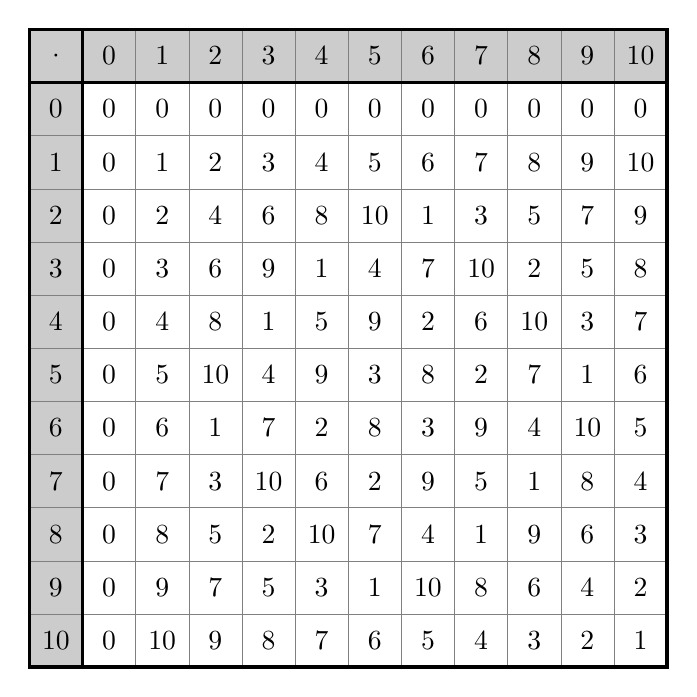
\begin{tikzpicture}[>=latex,thick,scale=0.45]
		\fill[color=gray!40] (0,0) rectangle (18,-1.5);
		\fill[color=gray!40] (0,0) rectangle (1.5,-18);	
		\draw[step = 1.5, gray,very thin] (0,0) grid (18,-18);
		\draw[very thick] (0,0) rectangle (18,-18);
		\draw[very thick] (0,-1.5) -- (18,-1.5);
		\draw[very thick] (1.5,0) -- (1.5,-18);
		\node at (0.75,-0.75) {$\cdot$};
		\foreach \x in {0,...,10}
		\node at (2.25+\x*1.5,-0.75) {$\x$};
		\foreach \y in {0,...,10}
		\node at (0.75,-2.25+\y*-1.5) {$\y$};
		% Row 0
		\node at ( 2.25,-2.25) {$0$};
		\node at ( 3.75,-2.25) {$0$};
		\node at ( 5.25,-2.25) {$0$};
		\node at ( 6.75,-2.25) {$0$};
		\node at ( 8.25,-2.25) {$0$};
		\node at ( 9.75,-2.25) {$0$};
		\node at (11.25,-2.25) {$0$};
		\node at (12.75,-2.25) {$0$};
		\node at (14.25,-2.25) {$0$};
		\node at (15.75,-2.25) {$0$};
		\node at (17.25,-2.25) {$0$};
		% Row 1
		\node at ( 2.25,-3.75) {$0$};
		\node at ( 3.75,-3.75) {$1$};
		\node at ( 5.25,-3.75) {$2$};
		\node at ( 6.75,-3.75) {$3$};
		\node at ( 8.25,-3.75) {$4$};
		\node at ( 9.75,-3.75) {$5$};
		\node at (11.25,-3.75) {$6$};
		\node at (12.75,-3.75) {$7$};
		\node at (14.25,-3.75) {$8$};
		\node at (15.75,-3.75) {$9$};
		\node at (17.25,-3.75) {$10$};
		% Row 2
		\node at ( 2.25,-5.25) {$0$};
		\node at ( 3.75,-5.25) {$2$};
		\node at ( 5.25,-5.25) {$4$};
		\node at ( 6.75,-5.25) {$6$};
		\node at ( 8.25,-5.25) {$8$};
		\node at ( 9.75,-5.25) {$10$};
		\node at (11.25,-5.25) {$1$};
		\node at (12.75,-5.25) {$3$};
		\node at (14.25,-5.25) {$5$};
		\node at (15.75,-5.25) {$7$};
		\node at (17.25,-5.25) {$9$};
		% Row 3
		\node at ( 2.25,-6.75) {$0$};
		\node at ( 3.75,-6.75) {$3$};
		\node at ( 5.25,-6.75) {$6$};
		\node at ( 6.75,-6.75) {$9$};
		\node at ( 8.25,-6.75) {$1$};
		\node at ( 9.75,-6.75) {$4$};
		\node at (11.25,-6.75) {$7$};
		\node at (12.75,-6.75) {$10$};
		\node at (14.25,-6.75) {$2$};
		\node at (15.75,-6.75) {$5$};
		\node at (17.25,-6.75) {$8$};
		% Row 4
		\node at ( 2.25,-8.25) {$0$};
		\node at ( 3.75,-8.25) {$4$};
		\node at ( 5.25,-8.25) {$8$};
		\node at ( 6.75,-8.25) {$1$};
		\node at ( 8.25,-8.25) {$5$};
		\node at ( 9.75,-8.25) {$9$};
		\node at (11.25,-8.25) {$2$};
		\node at (12.75,-8.25) {$6$};
		\node at (14.25,-8.25) {$10$};
		\node at (15.75,-8.25) {$3$};
		\node at (17.25,-8.25) {$7$};
		% Row 5
		\node at ( 2.25,-9.75) {$0$};
		\node at ( 3.75,-9.75) {$5$};
		\node at ( 5.25,-9.75) {$10$};
		\node at ( 6.75,-9.75) {$4$};
		\node at ( 8.25,-9.75) {$9$};
		\node at ( 9.75,-9.75) {$3$};
		\node at (11.25,-9.75) {$8$};
		\node at (12.75,-9.75) {$2$};
		\node at (14.25,-9.75) {$7$};
		\node at (15.75,-9.75) {$1$};
		\node at (17.25,-9.75) {$6$};
		% Row 6
		\node at ( 2.25,-11.25) {$0$};
		\node at ( 3.75,-11.25) {$6$};
		\node at ( 5.25,-11.25) {$1$};
		\node at ( 6.75,-11.25) {$7$};
		\node at ( 8.25,-11.25) {$2$};
		\node at ( 9.75,-11.25) {$8$};
		\node at (11.25,-11.25) {$3$};
		\node at (12.75,-11.25) {$9$};
		\node at (14.25,-11.25) {$4$};
		\node at (15.75,-11.25) {$10$};
		\node at (17.25,-11.25) {$5$};
		% Row 7
		\node at ( 2.25,-12.75) {$0$};
		\node at ( 3.75,-12.75) {$7$};
		\node at ( 5.25,-12.75) {$3$};
		\node at ( 6.75,-12.75) {$10$};
		\node at ( 8.25,-12.75) {$6$};
		\node at ( 9.75,-12.75) {$2$};
		\node at (11.25,-12.75) {$9$};
		\node at (12.75,-12.75) {$5$};
		\node at (14.25,-12.75) {$1$};
		\node at (15.75,-12.75) {$8$};
		\node at (17.25,-12.75) {$4$};
		% Row 8
		\node at ( 2.25,-14.25) {$0$};
		\node at ( 3.75,-14.25) {$8$};
		\node at ( 5.25,-14.25) {$5$};
		\node at ( 6.75,-14.25) {$2$};
		\node at ( 8.25,-14.25) {$10$};
		\node at ( 9.75,-14.25) {$7$};
		\node at (11.25,-14.25) {$4$};
		\node at (12.75,-14.25) {$1$};
		\node at (14.25,-14.25) {$9$};
		\node at (15.75,-14.25) {$6$};
		\node at (17.25,-14.25) {$3$};
		% Row 9
		\node at ( 2.25,-15.75) {$0$};
		\node at ( 3.75,-15.75) {$9$};
		\node at ( 5.25,-15.75) {$7$};
		\node at ( 6.75,-15.75) {$5$};
		\node at ( 8.25,-15.75) {$3$};
		\node at ( 9.75,-15.75) {$1$};
		\node at (11.25,-15.75) {$10$};
		\node at (12.75,-15.75) {$8$};
		\node at (14.25,-15.75) {$6$};
		\node at (15.75,-15.75) {$4$};
		\node at (17.25,-15.75) {$2$};
		% Row 10
		\node at ( 2.25,-17.25) {$0$};
		\node at ( 3.75,-17.25) {$10$};
		\node at ( 5.25,-17.25) {$9$};
		\node at ( 6.75,-17.25) {$8$};
		\node at ( 8.25,-17.25) {$7$};
		\node at ( 9.75,-17.25) {$6$};
		\node at (11.25,-17.25) {$5$};
		\node at (12.75,-17.25) {$4$};
		\node at (14.25,-17.25) {$3$};
		\node at (15.75,-17.25) {$2$};
		\node at (17.25,-17.25) {$1$};
	\end{tikzpicture}
	
\end{center}

Die Menge uns zur Verfügung stehender Zahlen legt auch fest, wie viele Zahlen ein Nachrichtenblock $n$, bestehend aus Nutzdatenteil und Fehlerkorrekturteil, umfassen kann.
Der Nachrichtenblock im Beispiel besteht aus
\[
n = q - 1 = 10 \text{ Zahlen},
\]
wobei die Null weggelassen wird. Wenn wir versuchen würden, mit der Null zu codieren, stellen wir fest, dass wir wieder null an der gleichen Stelle erhalten und somit wäre die Codierung nicht eindeutig.

% Notes
%Da bei allen Codes, die codiert werden wird an der gleichen Stelle eine Nullstelle auftreten.

% Old Text
%Die grösse des endlichen Körpers legt auch fest, wie gross unsere Nachricht $n$ bestehend aus Nutzdatenteil und Fehlerkorrekturteil sein kann und beträgt in unserem Beispiel
%\[
%n = q - 1 = 10 \text{ Zahlen}.
%\]

Im nächsten Schritt bestimmen wir, wie viele Fehler $t$ während der Übertragung maximal auftreten dürfen, damit wir sie noch korrigieren können.
Unser Beispielcode sollte in der Lage sein
\[
t = 2
\]
Fehlerstellen korrigieren zu können.

Die Grösse des Nutzdatenteils hängt von der Grösse des Nachrichtenblocks sowie der Anzahl der Fehlerkorrekturstellen ab. Je robuster der Code sein muss, desto weniger Platz bleibt für Nutzdaten $k$ in der Nachricht übrig.
Bei maximal 2 Fehlern können wir noch
\[
k = n - 2t = 6\text{ Zahlen}
\]
übertragen. 

Zusammenfassend haben wir einen Nachrichtenblock mit der Länge von 10 Zahlen definiert, der 6 Zahlen als Nutzlast beinhaltet und in der Lage ist, aus 2 fehlerhaften Stellen im Block die ursprünglichen Nutzdaten zu rekonstruieren. Zudem werden wir im Weiteren feststellen, dass dieser Code maximal vier Fehlerstellen erkennen, diese aber nicht rekonstruieren kann.

Wir legen nun für das Beispiel die Nachricht
\[
m = [0,0,0,0,4,7,2,5,8,1]
\]
fest, die wir gerne an einen Empfänger übertragen möchten, wobei die vorderen vier Stellen für die Fehlerkorrektur zuständig sind.
Solange diese Stellen vor dem Codieren und nach dem Decodieren den Wert null haben, ist die Nachricht fehlerfrei übertragen worden.

Da wir in den folgenden Abschnitten mit Polynomen arbeiten, stellen wir die Nachricht auch noch als Polynom
\[
m(X) = 4X^5 + 7X^4 + 2X^3 + 5X^2 + 8X + 1
\] 
dar.

% Old Text
%Die Nachricht können wir auch als Polynom 
%\[
%m(X) = 4X^5 + 7X^4 + 2X^3 + 5X^2 + 8X + 1
%\] 
%darstellen.

\subsection{Der Ansatz der diskreten Fouriertransformation
	\label{reedsolomon:subsection:diskFT}}

Im vorherigen Abschnitt \ref{reedsolomon:section:dtf} haben wir schon einmal die diskrete Fouriertransformation zum Codieren einer Nachricht verwendet. In den endlichen Körpern wird dies jedoch nicht gelingen, da die Eulersche Zahl $e$ in endlichen Körpern nicht existiert.
Wir wählen deshalb eine Zahl $a$, die die gleiche Aufgabe haben soll wie $e^{\frac{j}{2 \pi}}$ in der diskreten Fouriertransformation, nur mit dem Unterschied, dass $a$ in $\mathbb{F}_{11}$ ist. Dazu soll die Potenz von $a$ den gesamten Zahlenbereich von $\mathbb{F}_{11}$ abdecken.
Dazu ändern wir die Darstellung von
\[
\mathbb{F}_{11} = \{0,1,2,3,4,5,6,7,8,9,10\}
\]
in die von $a$ abhängige Schreibweise 
\[
\mathbb{Z}_{11}\setminus\{0\} = \{a^0, a^1, a^2, a^3, a^4, a^5, a^6, a^7, a^8, a^9\}.
\]
%Jetzt brauchen wir nur noch eine geeignete Zahl für $a$ zu finden.
% Old Text
%Wir suchen also eine Zahl $a$, die in endlichen Körpern existiert und den gesamten Zahlenbereich von $\mathbb{F}_{11}$ abdecken kann.
%Dazu schreiben wir
%\[
%\mathbb{F}_{11} = \{0,1,2,3,4,5,6,7,8,9,10\}
%\]
%um in 
%\[
%\mathbb{Z}_{11}\setminus\{0\} = \{a^0, a^1, a^2, a^3, a^4, a^5, a^6, a^7, a^8, a^9\}.
%\]
%
%Wenn wir alle möglichen Werte für $a$ einsetzen, also
%\begin{align}
%a = 0 : \qquad \mathbb{Z}_{11}\setminus\{0\} = \{0, 0, 0, 0, 0, 0, 0, 0, 0, 0\} \\
%a = 1 : \qquad \mathbb{Z}_{11}\setminus\{0\} = \{1, 1, 1, 1, 1, 1, 1, 1, 1, 1\} \\
%a = 2 : \qquad \mathbb{Z}_{11}\setminus\{0\} = \{1, 2, 4, 8, 5, 10, 9, 7, 3, 6\} \\
%a = 3 : \qquad \mathbb{Z}_{11}\setminus\{0\} = \{1, 3, 9, 5, 4, 1, 3, 9, 5, 4\} \\
%a = 4 : \qquad \mathbb{Z}_{11}\setminus\{0\} = \{1, 4, 5, 9, 3, 1, 4, 5, 9, 3\} \\
%a = 5 : \qquad \mathbb{Z}_{11}\setminus\{0\} = \{1, 5, 3, 4, 9, 1, 5, 3, 4, 9\} \\
%a = 6 : \qquad \mathbb{Z}_{11}\setminus\{0\} = \{1, 6, 3, 7, 9, 10, 5, 8, 4, 2\} \\
%a = 7 : \qquad \mathbb{Z}_{11}\setminus\{0\} = \{1, 7, 5, 2, 3, 10, 4, 6, 9, 8\} \\
%a = 8 : \qquad \mathbb{Z}_{11}\setminus\{0\} = \{1, 8, 9, 6, 4, 10, 3, 2, 5, 7\} \\
%a = 9 : \qquad \mathbb{Z}_{11}\setminus\{0\} = \{1, 9, 4, 3, 5, 1, 9, 4, 3, 5\} \\
%a = 10 : \qquad \mathbb{Z}_{11}\setminus\{0\} = \{1, 10, 1, 10, 1, 10, 1, 10, 1, 10\}
%\end{align}

\subsubsection{Die primitiven Einheitswurzeln
	\label{reedsolomon:subsection:primsqrt}}
\index{primitive Einheitswurzel}%
\index{Einheitswurzel, primitiv}%
Wenn wir jetzt Zahlen von $\mathbb{F}_{11}$ an Stelle von $a$ einsetzen, erhalten wir
\begin{center}
\def\s{\phantom{0}}
\begin{tabular}{c c c c c c l}
$a = \s1$ & $\Rightarrow$ & $\{a^i | 0 \le i \le 10\}$ & $=$ & $\{1,\s1,\s1,\s1,\s1,\s1,\s1,\s1,\s1,\s1\}$ & $\neq$ & $\mathbb{F}_{11}\setminus\{0\}$ \\
$a = \s2$ & $\Rightarrow$ & $\{a^i | 0 \le i \le 10\}$ & $=$ & $\{1,\s2,\s4,\s8,\s5,10,\s9,\s7,\s3,\s6\}$ & $ = $ & $\mathbb{F}_{11}\setminus\{0\}$ \\
$a = \s3$ & $\Rightarrow$ & $\{a^i | 0 \le i \le 10\}$ & $=$ & $\{1,\s3,\s9,\s5,\s4,\s1,\s3,\s9,\s5,\s4\}$ & $\neq$ & $\mathbb{F}_{11}\setminus\{0\}$ \\
$a = \s4$ & $\Rightarrow$ & $\{a^i | 0 \le i \le 10\}$ & $=$ & $\{1,\s4,\s5,\s9,\s3,\s1,\s4,\s5,\s9,\s3\}$ & $\neq$ & $\mathbb{F}_{11}\setminus\{0\}$ \\
$a = \s5$ & $\Rightarrow$ & $\{a^i | 0 \le i \le 10\}$ & $=$ & $\{1,\s5,\s3,\s4,\s9,\s1,\s5,\s3,\s4,\s9\}$ & $\neq$ & $\mathbb{F}_{11}\setminus\{0\}$ \\
$a = \s6$ & $\Rightarrow$ & $\{a^i | 0 \le i \le 10\}$ & $=$ & $\{1,\s6,\s3,\s7,\s9, 10,\s5,\s8,\s4,\s2\}$ & $ = $ & $\mathbb{F}_{11}\setminus\{0\}$ \\
$a = \s7$ & $\Rightarrow$ & $\{a^i | 0 \le i \le 10\}$ & $=$ & $\{1,\s7,\s5,\s2,\s3,10,\s4,\s6,\s9,\s8\}$ & $ = $ & $\mathbb{F}_{11}\setminus\{0\}$ \\
$a = \s8$ & $\Rightarrow$ & $\{a^i | 0 \le i \le 10\}$ & $=$ & $\{1,\s8,\s9,\s6,\s4, 10,\s3,\s2,\s5,\s7\}$ & $ = $ & $\mathbb{F}_{11}\setminus\{0\}$ \\
$a = \s9$ & $\Rightarrow$ & $\{a^i | 0 \le i \le 10\}$ & $=$ & $\{1,\s9,\s4,\s3,\s5,\s1,\s9,\s4,\s3,\s5\}$ & $\neq$ & $\mathbb{F}_{11}\setminus\{0\}$ \\
$a = 10$ & $\Rightarrow$ & $\{a^i | 0 \le i \le 10\}$ & $=$ & $\{1, 10,\s1,10,\s1, 10,\s1, 10,\s1, 10\}$ & $\neq$ & $\mathbb{F}_{11}\setminus\{0\}$. \\
\end{tabular}
\end{center}
%\begin{center}
%\begin{tabular}{c r c l}
%%$a = 0 :$& $\qquad \mathbb{Z}_{11}\setminus\{0\}$ &$=$& $\{0, 0, 0, 0, 0, 0, 0, 0, 0, 0\}$ \\
%$a = 1 :$& $\qquad \mathbb{Z}_{11}\setminus\{0\}$ &$=$& $\{1, 1, 1, 1, 1, 1, 1, 1, 1, 1\}$ \\
%$a = 2 :$& $\qquad \mathbb{Z}_{11}\setminus\{0\}$ &$=$& $\{1, 2, 4, 8, 5, 10, 9, 7, 3, 6\}$ \\
%$a = 3 :$& $\qquad \mathbb{Z}_{11}\setminus\{0\}$ &$=$& $\{1, 3, 9, 5, 4, 1, 3, 9, 5, 4\}$ \\
%$a = 4 :$& $\qquad \mathbb{Z}_{11}\setminus\{0\}$ &$=$& $\{1, 4, 5, 9, 3, 1, 4, 5, 9, 3\}$ \\
%$a = 5 :$& $\qquad \mathbb{Z}_{11}\setminus\{0\}$ &$=$& $\{1, 5, 3, 4, 9, 1, 5, 3, 4, 9\}$ \\
%$a = 6 :$& $\qquad \mathbb{Z}_{11}\setminus\{0\}$ &$=$& $\{1, 6, 3, 7, 9, 10, 5, 8, 4, 2\}$ \\
%$a = 7 :$& $\qquad \mathbb{Z}_{11}\setminus\{0\}$ &$=$& $\{1, 7, 5, 2, 3, 10, 4, 6, 9, 8\}$ \\
%$a = 8 :$& $\qquad \mathbb{Z}_{11}\setminus\{0\}$ &$=$& $\{1, 8, 9, 6, 4, 10, 3, 2, 5, 7\}$ \\
%$a = 9 :$& $\qquad \mathbb{Z}_{11}\setminus\{0\}$ &$=$& $\{1, 9, 4, 3, 5, 1, 9, 4, 3, 5\}$ \\
%$a = 10 :$& $\qquad \mathbb{Z}_{11}\setminus\{0\}$ &$=$& $\{1, 10, 1, 10, 1, 10, 1, 10, 1, 10\}$	
%\end{tabular}
%\end{center}
Es fällt auf, dass wir für $a$ die Zahlen $2,6,7,8$ Mengen erhalten, die tatsächlich den gesamten Zahlenraum von $\mathbb{F}_{11}$ abbilden. Solche Zahlen werden \em primitive Einheitswurzeln \em genannt. 
Wenden wir diese Vorgehensweise auch für andere endliche Körper an, so werden wir sehen, dass wir immer mindestens zwei solcher Einheitswurzeln finden werden. Somit ist es uns überlassen, eine dieser Einheitswurzeln auszuwählen, mit der wir weiter rechnen wollen. Für das Beispiel wählen wir die Zahl $a = 8$.

\subsubsection{Bildung einer Transformationsmatrix
	\label{reedsolomon:subsection:transMat}}
\index{Transformationsmatrix}%

Mit der Wahl einer Einheitswurzel ist es uns jetzt möglich, unsere Nachricht zu codieren. Daraus sollen wir dann einen Übertragungsvektor $v$ erhalten, den wir an den Empfänger schicken können. 
Für die Codierung setzen wir alle Zahlen in $\mathbb{F}_{11}\setminus\{0\}$ nacheinander in $m(X)$ ein. Da wir zuvor eine von $a$ abhängige Schreibweise gewählt haben, setzen wir stattdessen $a^i$ ein mit $a = 8$ als die von uns gewählten primitiven Einheitswurzel. Daraus ergibt sich
%Für die Codierung müssen wir alle $a^i$ in das Polynom $m(X)$ einsetzen. Da wir $a^i = 8^i$ gewählt haben, ergibt sich daraus 
%
%Damit wir unsere Nachricht codieren können, müssen wir $8^i$ in $m(X)$ einsetzen.
%
\begin{center}
	\begin{tabular}{c}
		$m(8^0) = 4 \cdot 1^5 + 7 \cdot 1^4 + 2 \cdot 1^3 + 5 \cdot 1^2 + 8 \cdot 1^1 + 1 = 5$ \\
		$m(8^1) = 4 \cdot 8^5 + 7 \cdot 8^4 + 2 \cdot 8^3 + 5 \cdot 8^2 + 8 \cdot 8^1 + 1 = 3$ \\
		\vdots \\[5pt]
		$m(8^9) = 4 \cdot 7^5 + 7 \cdot 7^4 + 2 \cdot 7^3 + 5 \cdot 7^2 + 8 \cdot 7^1 + 1 = 4$
	\end{tabular}
\end{center}
als unser Übertragungsvektor. 
\index{Ubertragungsvektor@Übertragungsvektor}%

\subsection{Allgemeine Codierung
	\label{reedsolomon:subsection:algCod}}
Um das Ganze noch ein wenig übersichtlicher zu gestalten, können wir die Polynome zu einer Matrix zusammenfassen, die unsere Transformationsmatrix $A$ bildet.

Für die allgemeine Codierung benötigen wir die Nachricht $m$, die codiert werden soll sowie die Transformationsmatrix $A$. Daraus erhalten wir den Übertragungsvektor $v$. Setzen wir die Zahlen aus dem Beispiel ein, erhalten wir folgende Darstellung:
\[
v = A \cdot m \qquad \Rightarrow \qquad v = \begin{pmatrix}
	8^0&    8^0&    8^0&    8^0&    8^0&    8^0&    8^0&    8^0&    8^0&    8^0\\
	8^0&	8^1&	8^2&	8^3&	8^4&	8^5&	8^6&	8^7&    8^8&	8^9\\
	8^0&	8^2&	8^4&	8^6&	8^8& 8^{10}& 8^{12}& 8^{14}& 8^{16}& 8^{18}\\
	8^0&	8^3&	8^6&	8^9& 8^{12}& 8^{15}& 8^{18}& 8^{21}& 8^{24}& 8^{27}\\
	8^0&	8^4&	8^8& 8^{12}& 8^{16}& 8^{20}& 8^{24}& 8^{28}& 8^{32}& 8^{36}\\
	8^0&	8^5& 8^{10}& 8^{15}& 8^{20}& 8^{25}& 8^{30}& 8^{35}& 8^{40}& 8^{45}\\
	8^0&	8^6& 8^{12}& 8^{18}& 8^{24}& 8^{30}& 8^{36}& 8^{42}& 8^{48}& 8^{54}\\
	8^0&	8^7& 8^{14}& 8^{21}& 8^{28}& 8^{35}& 8^{42}& 8^{49}& 8^{56}& 8^{63}\\
	8^0&	8^8& 8^{16}& 8^{24}& 8^{32}& 8^{40}& 8^{48}& 8^{56}& 8^{64}& 8^{72}\\
	8^0&	8^9& 8^{18}& 8^{27}& 8^{36}& 8^{45}& 8^{54}& 8^{63}& 8^{72}& 8^{81}\\
\end{pmatrix}
\cdot
\begin{pmatrix}
	1 \\ 8 \\ 5 \\ 2 \\ 7 \\ 4 \\ 0 \\ 0 \\ 0 \\ 0 \\
\end{pmatrix}
.
\]
Für unseren Übertragungsvektor resultiert
\[
v = [5,3,6,5,2,10,2,7,10,4],
\]
den wir jetzt über einen beliebigen Nachrichtenkanal versenden können.
\index{Nachrichtenkanal}%
